 \documentclass{beamer}

\usepackage{graphicx}
\usepackage{ae}
\usepackage{multimedia}

\setbeamertemplate{footline}[frame number]


\newcommand{\info}[1]{{\footnotesize\textcolor{gray}{#1}}}
\newcommand{\unit}[2]{\ensuremath{#1\,\mathrm{#2}}}
\newcommand{\datawidth}{.43\textwidth}


\title{The Baxter Anomaly Data Set}
\author{Marvin Ludersdorfer}
\institute{Technische Universit\"{a}t M\"{u}nchen}
\date{}


\begin{document}

    \frame{\titlepage}

    \begin{frame}
    	\frametitle{Motivation}
        \begin{figure}
            \centering
            \includegraphics[width=\textwidth]{figs/robots}
        \end{figure}
        
        \vfill
        \begin{block}{Assumptions}
            \begin{itemize}
                \item motion is important part of any (robot) task
                \item<2-> anomaly in robot motion corresponds to change in dynamic behavior
            \end{itemize}
            \visible<2->{
                $\Rightarrow$ model anomalies as changes in robot control parameters
            }
    	\end{block}
    \end{frame}

    \begin{frame}
    	\frametitle{Experiment}
    	\begin{columns}[onlytextwidth]
            \begin{column}{.5\textwidth}
                \begin{block}{`normal' trial}
                    \vspace{.5\baselineskip}
                    \movie[width=.9\columnwidth,showcontrols=true]
                    {\includegraphics[width=.9\columnwidth]{figs/normal.png}}
                    {movs/normal.mp4}
                \end{block}
            \end{column}
            \begin{column}{.5\textwidth}
                \begin{block}{anomalous trial}
                    \vspace{.5\baselineskip}
                    \movie[width=.9\columnwidth,showcontrols=true]
                    {\includegraphics[width=.9\columnwidth]{figs/anomalous.png}}
                    {movs/anomalous.mp4}
                \end{block}
            \end{column}
        \end{columns}
    \end{frame}

    \begin{frame}
    	\frametitle{Data recorded}
        \begin{columns}[onlytextwidth]
            \begin{column}{.6\textwidth}
                \begin{itemize}
                    \item measured wrist acceleration \info{@ \unit{25}{Hz}}
                    \item commanded configuration \info{as it happens}
                    \item measured configuration \info{@ \unit{96}{Hz}}
                    \item generated torques \info{@ \unit{149}{Hz}}
                    \item commanded torques \info{@ \unit{96}{Hz}}
                    \item measured torques \info{@ \unit{96}{Hz}}
                    \item camera images \info{$320\times 200$ pixels @ \unit{25}{Hz}}
                \end{itemize}
            \end{column}
            \begin{column}{.4\textwidth}
                \begin{figure}
                    \centering
                    \includegraphics[width=.9\columnwidth]{figs/baxterjoints}
                \end{figure}
            \end{column}
        \end{columns}
    \end{frame}

    \begin{frame}
    	\frametitle{Data set structure}
        \begin{columns}[onlytextwidth]
            \begin{column}{.6\textwidth}
                Two data sets
                \begin{itemize}
                    \item `normal' \texttt{201508061628without.h5}
                    \item anomalous \texttt{201508071533with.h5}
                \end{itemize}
                contain each
                \begin{itemize}
                    \item trials $0, \ldots, 99$
                \end{itemize}
                where each trial contains
                \begin{itemize}
                    \item acceleration
                    \item configuration
                    \item effort
                    \item images
                \end{itemize}
                which in turn hold the mentioned data fields
            \end{column}
            \begin{column}{.4\textwidth}
                \begin{figure}
                    \centering
                    \includegraphics[width=.7\columnwidth]{figs/h5}
                \end{figure}
            \end{column}
        \end{columns}
    \end{frame}

    \begin{frame}
    	\frametitle{Looking at data: `Normal' data}
    	\begin{figure}
            \centering
            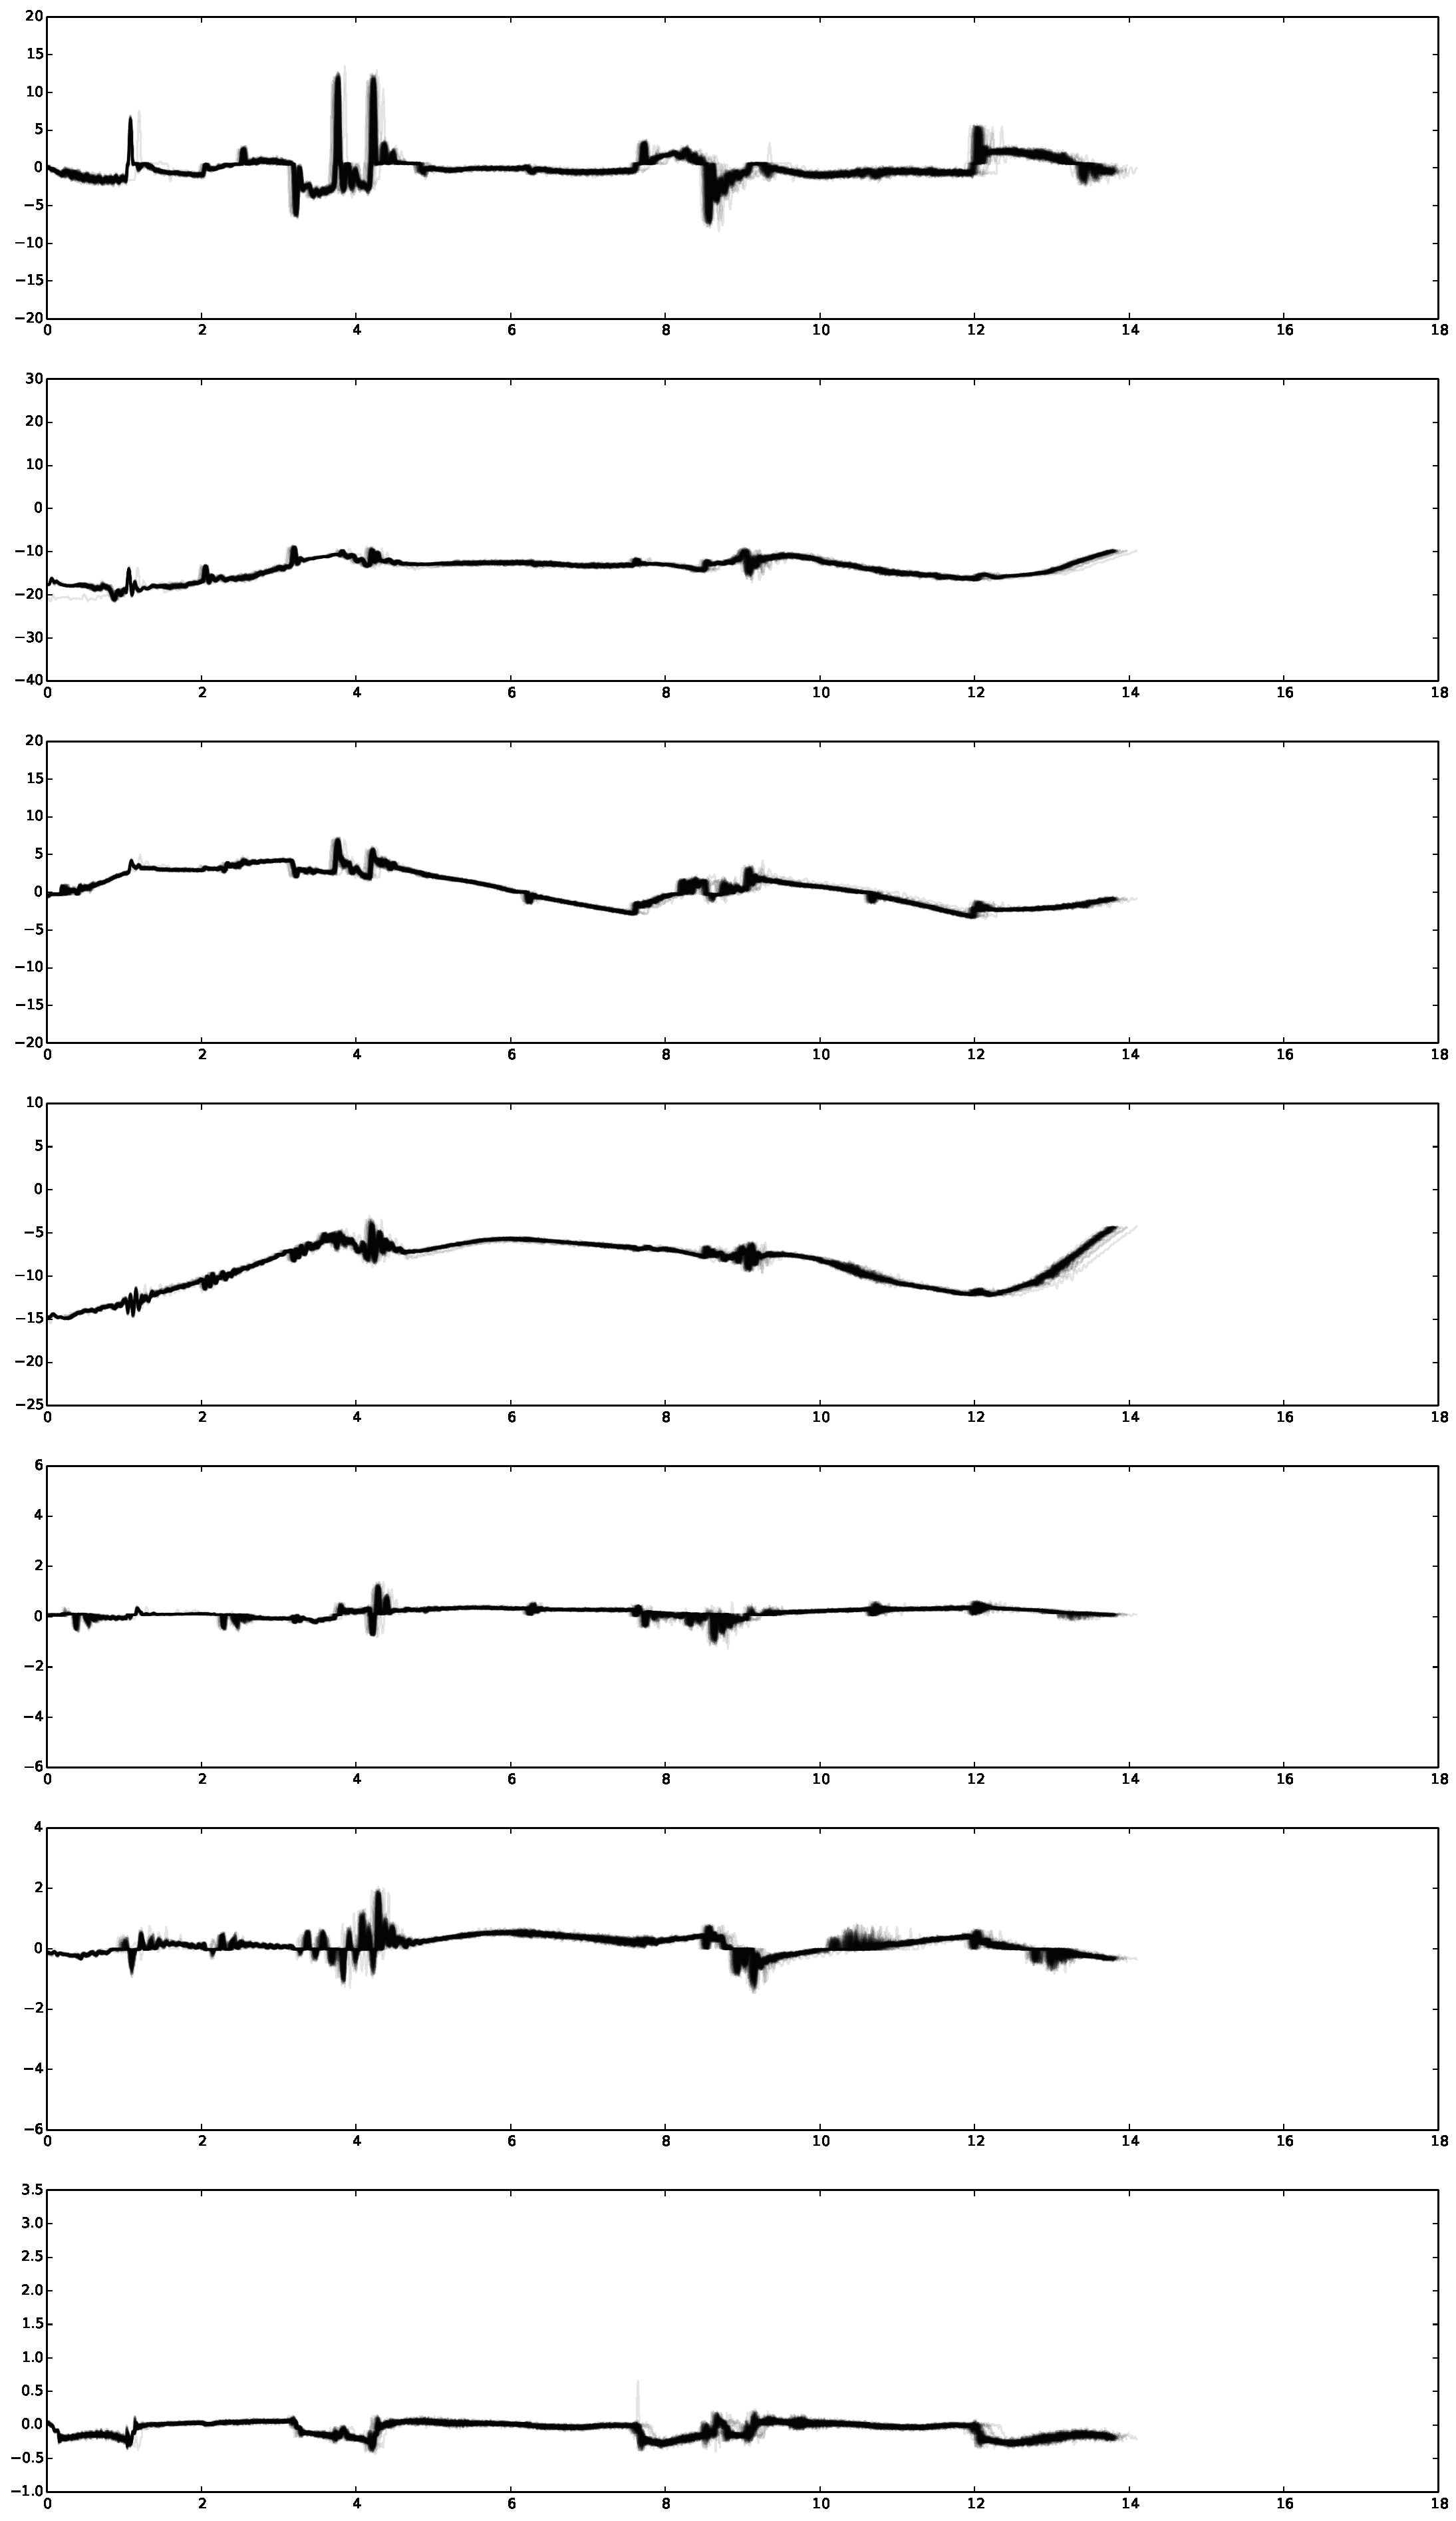
\includegraphics[width=\datawidth]{figs/no_anomaly3.png}
        \end{figure}
    \end{frame}

    \begin{frame}
        \frametitle{Looking at data: Anomalous data}
        \begin{figure}
            \centering
            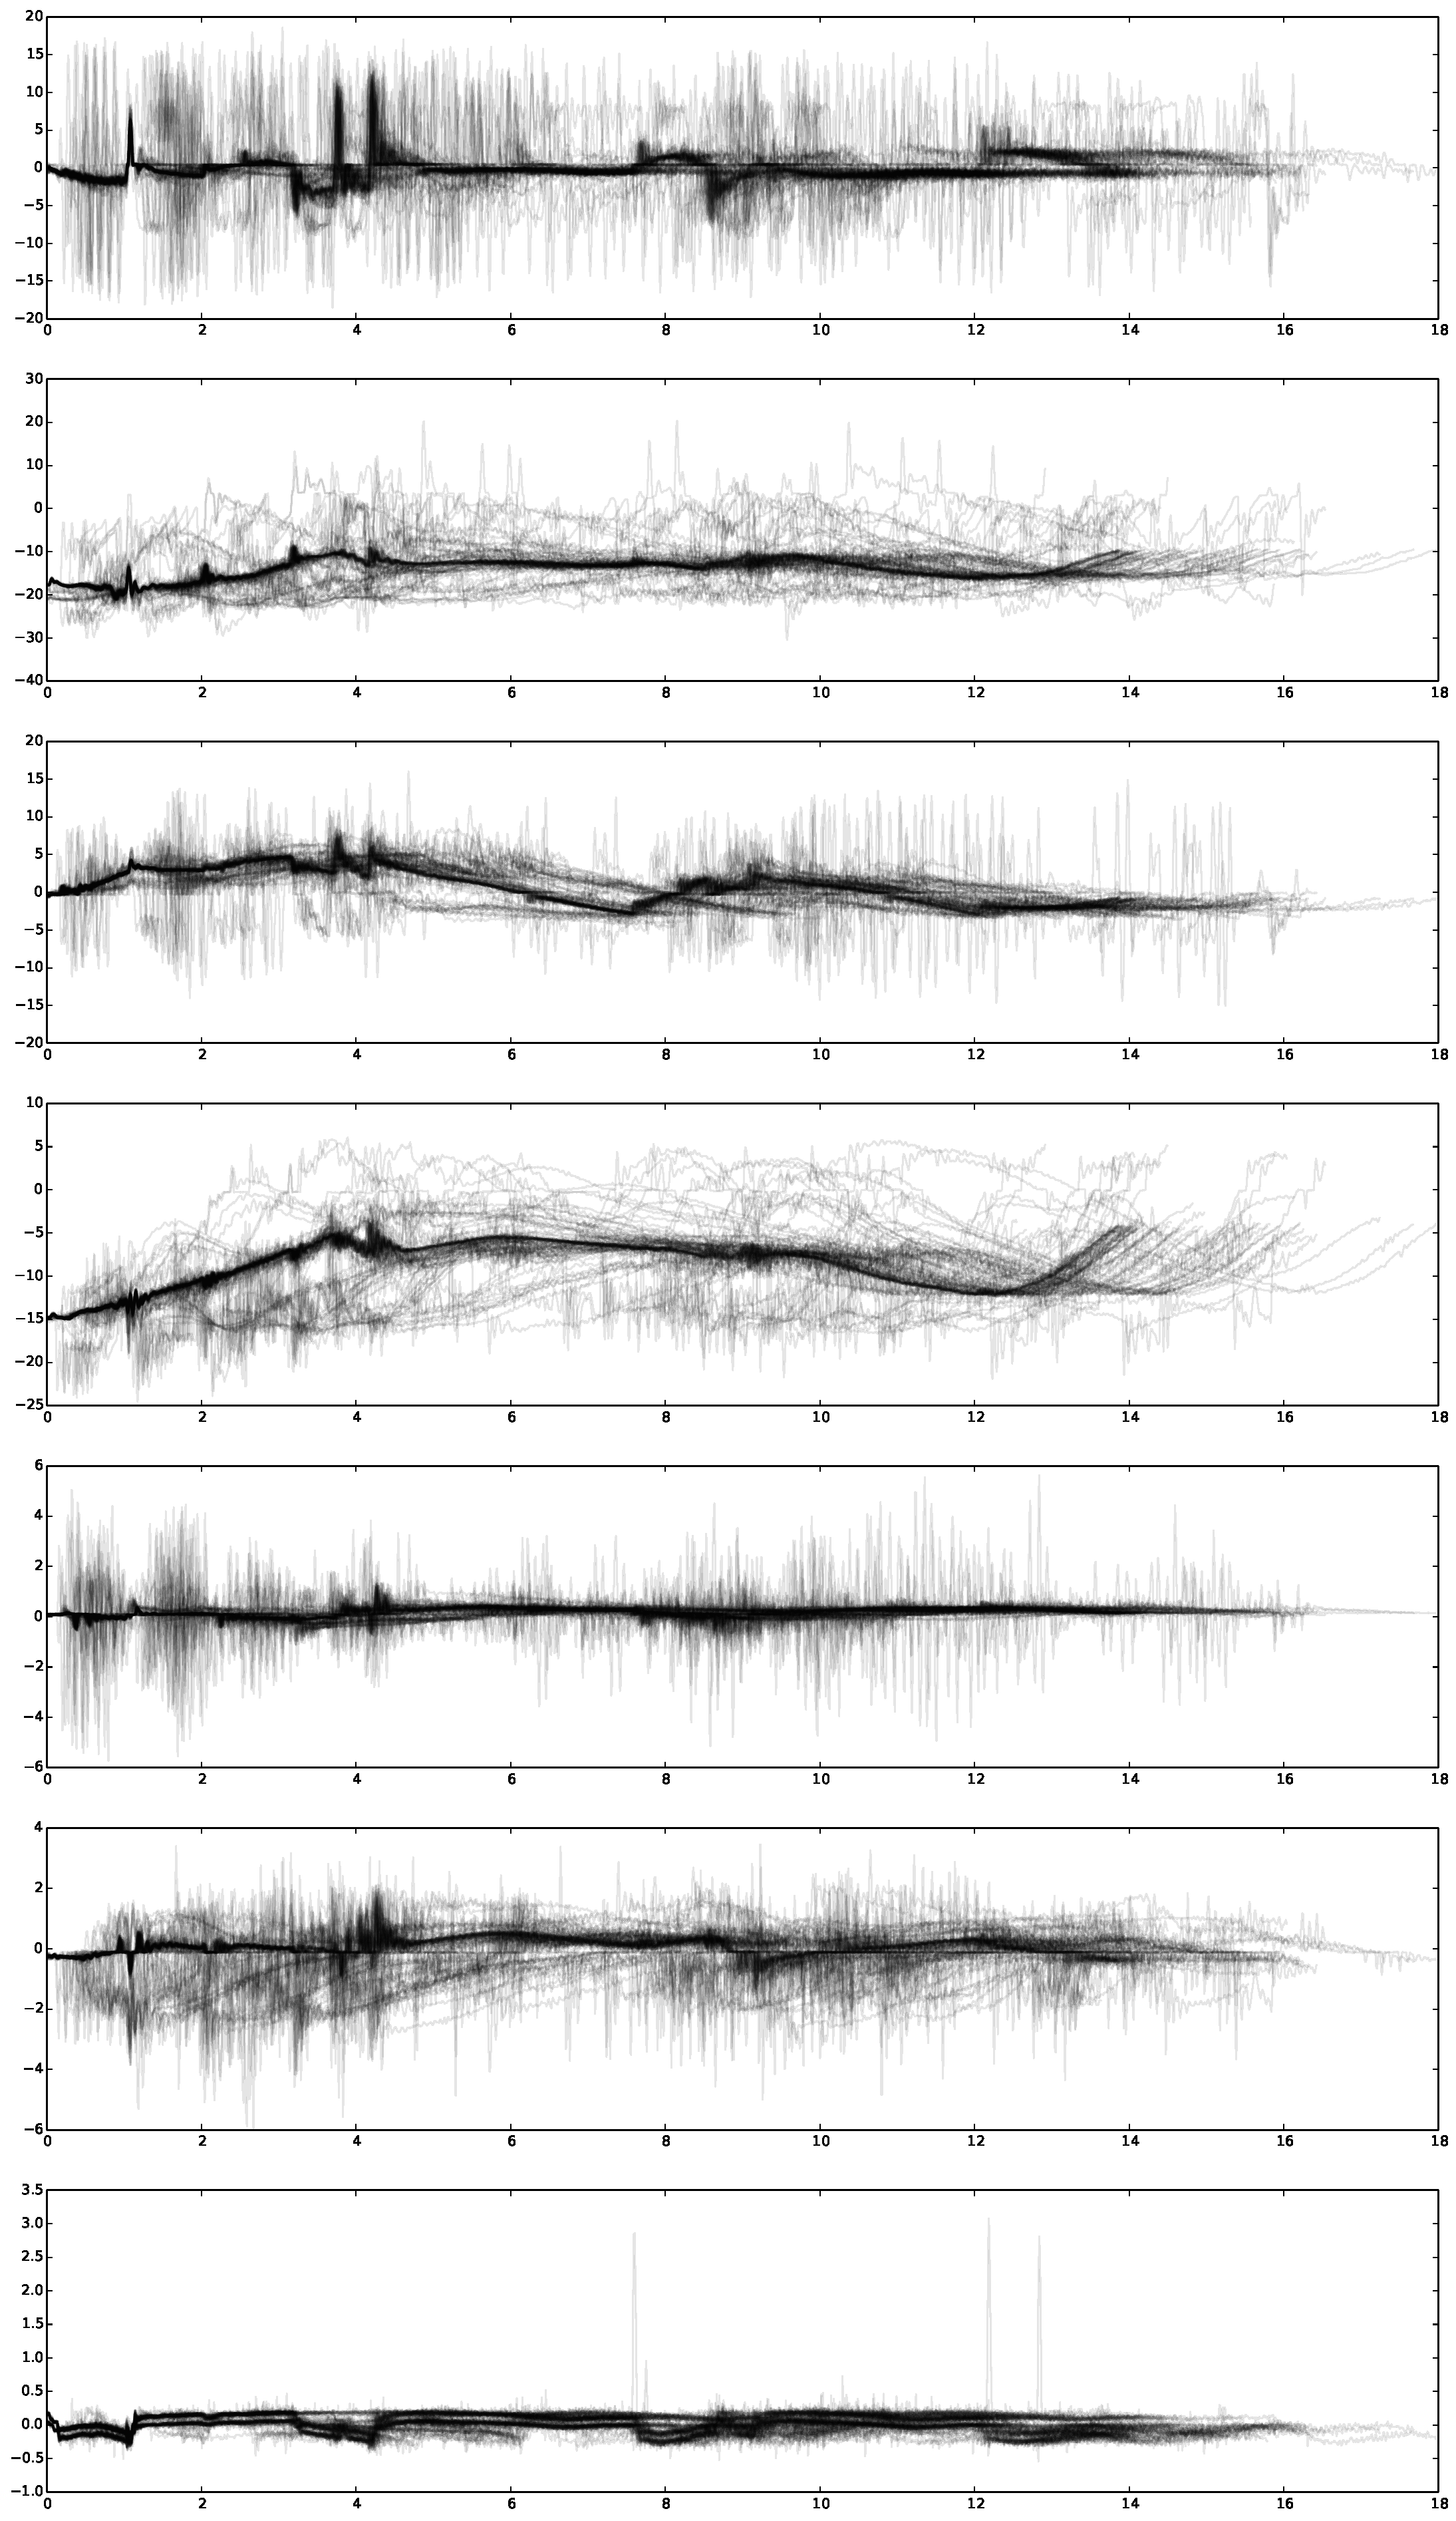
\includegraphics[width=\datawidth]{figs/controller_broke3.png}
        \end{figure}
    \end{frame}

    \begin{frame}
        \frametitle{Looking at data: Close-up anomaly data (1)}
        \begin{figure}
            \centering
            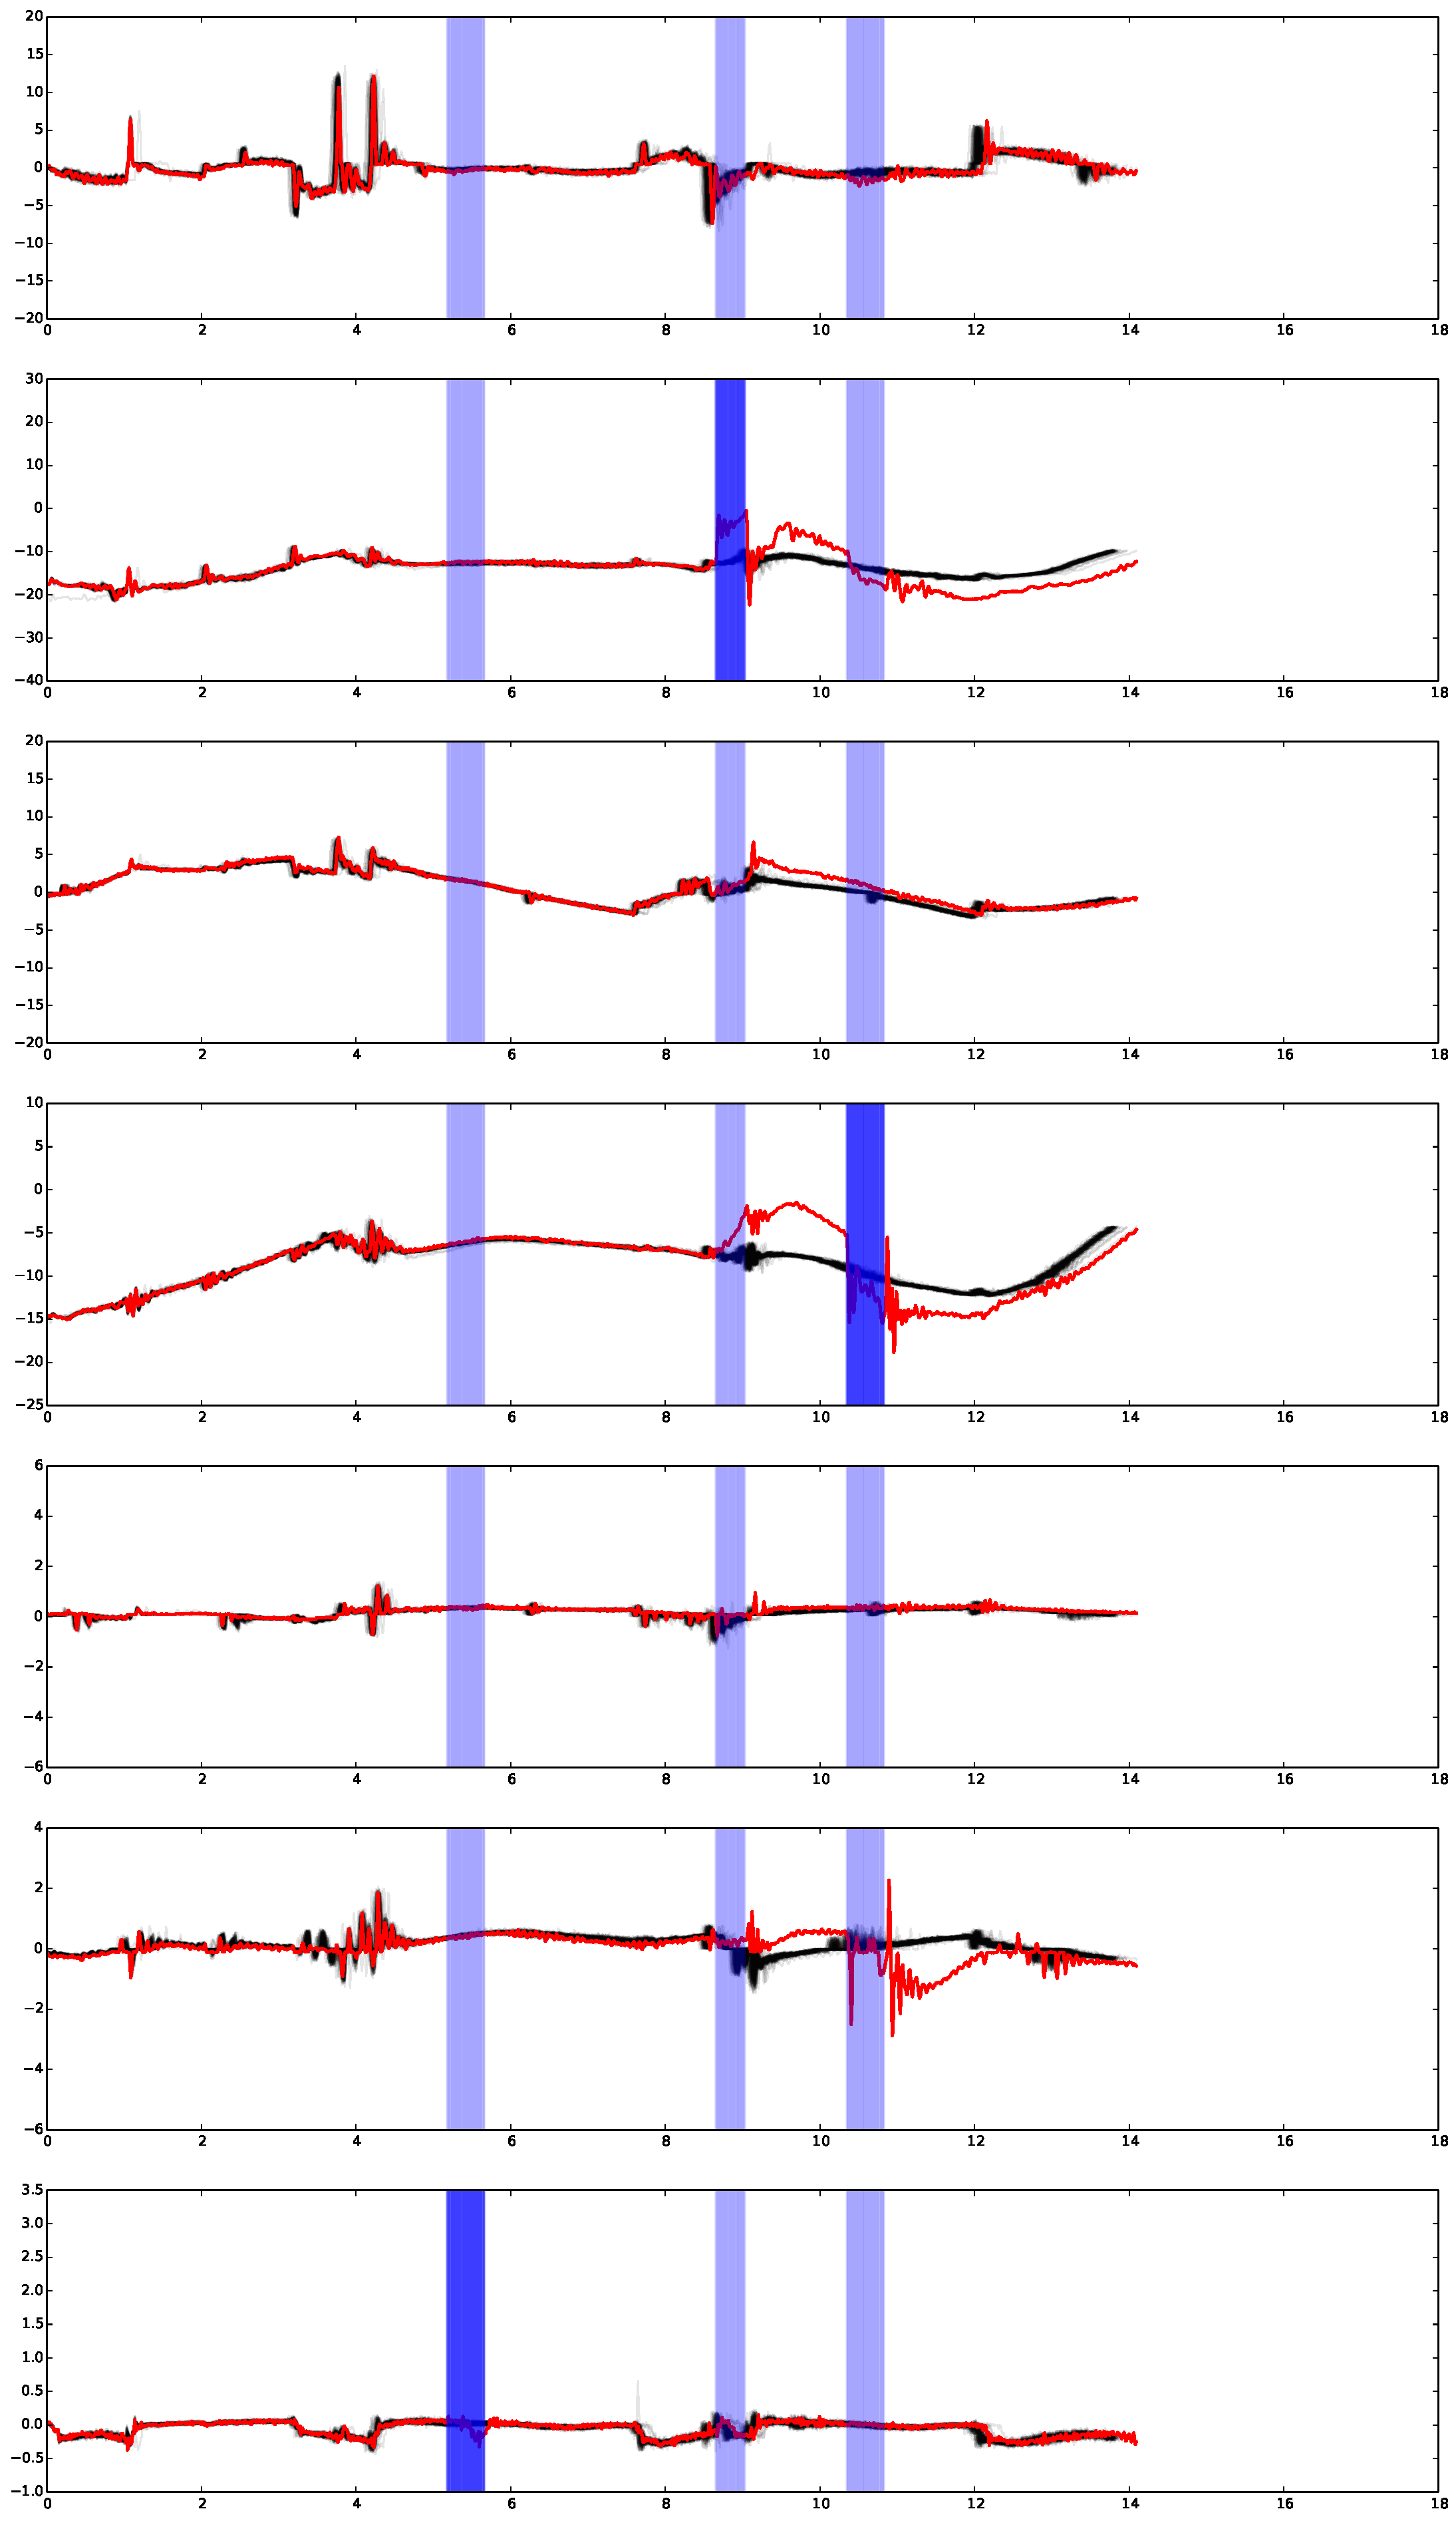
\includegraphics[width=\datawidth]{figs/anomaly12.png}
        \end{figure}
    \end{frame}

    \begin{frame}
        \frametitle{Looking at data: Close-up anomaly data (2)}
        \begin{figure}
            \centering
            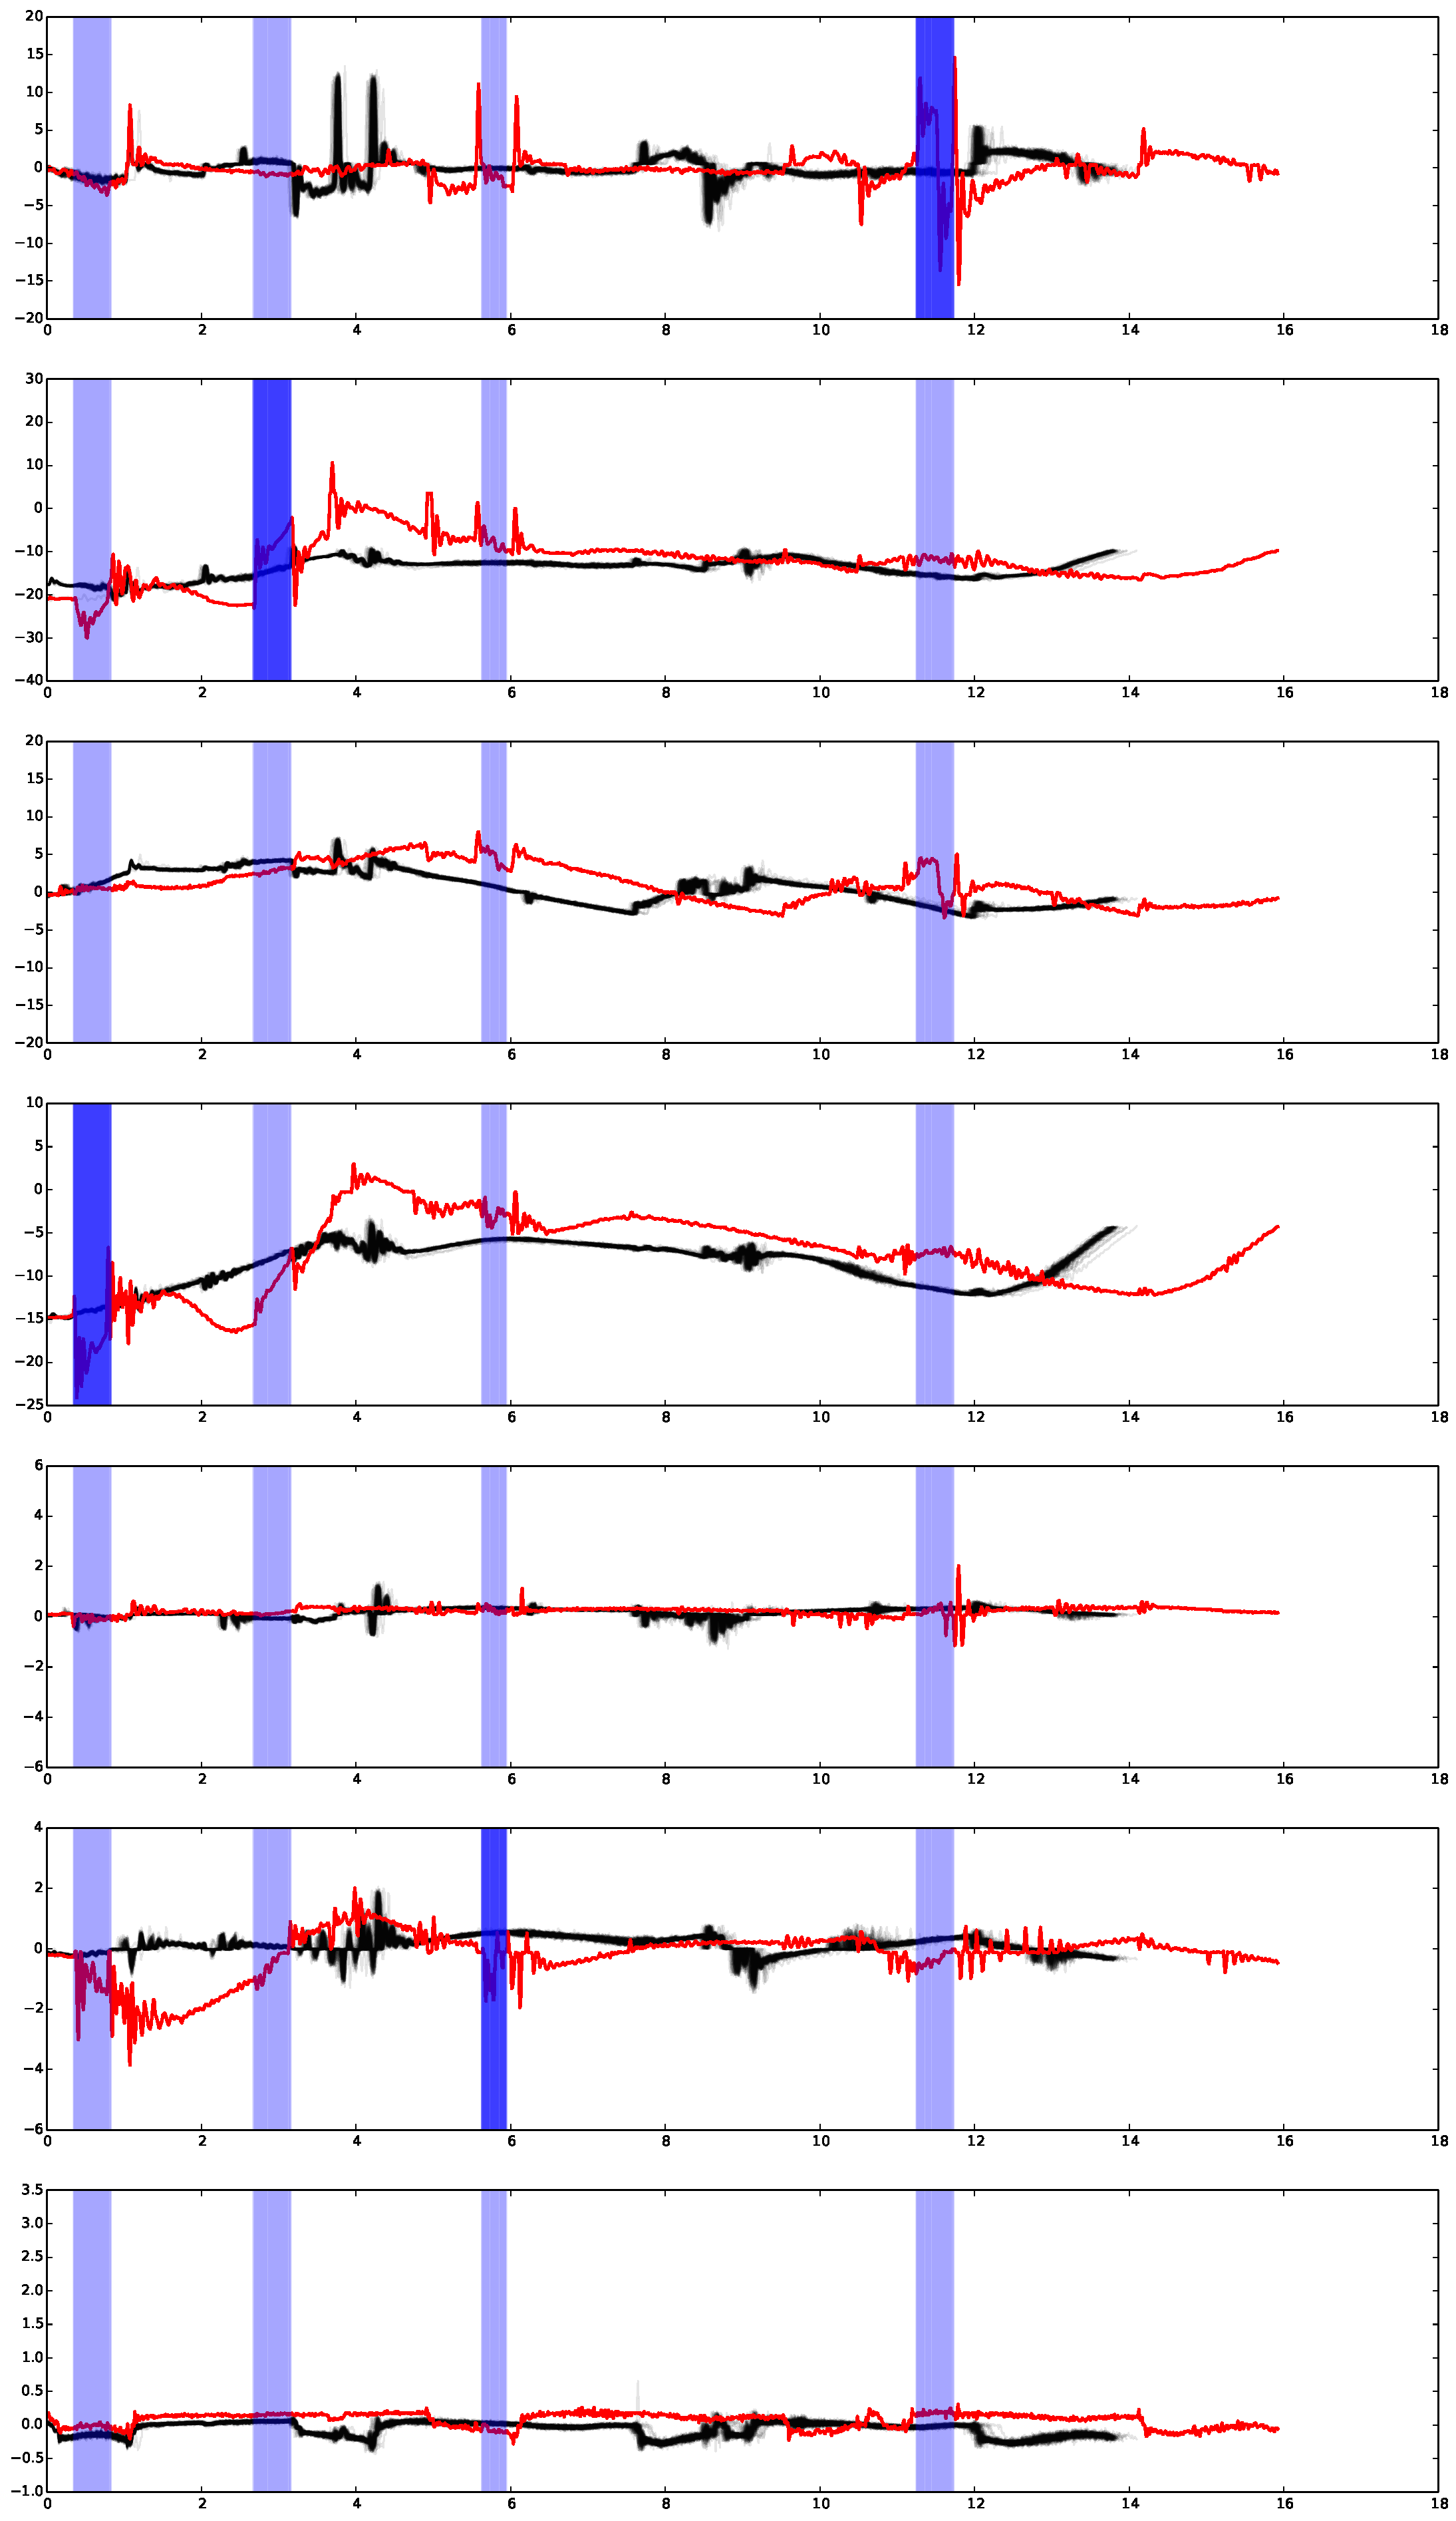
\includegraphics[width=\datawidth]{figs/anomaly50.png}
        \end{figure}
    \end{frame}

    \begin{frame}
        \frametitle{Where to get the data?}
        Go to \url{https://www.brml.tum.de/BaxterCollision}
        and log on with
        \begin{itemize}
            \item user: \texttt{AnomalyWeb@brml.tum.de}
            \item pwd: \texttt{hit\_Baxter01}
        \end{itemize}
        \vspace{1cm}
        The data we were looking at today is in
        \begin{itemize}
            \item `normal': \texttt{data/preliminary\_control/no\_anomaly\_3}
            \item anomalous: \texttt{data/preliminary\_control/controller\_broke\_3}
            \item plots: \texttt{data/preliminary\_control/Anomaly data nosing-no\_anomaly\_3\_+\_controller\_broke\_3.ipynb} 
        \end{itemize}
    \end{frame}

\end{document}
